\begin{figure*}[htbp]
\centering
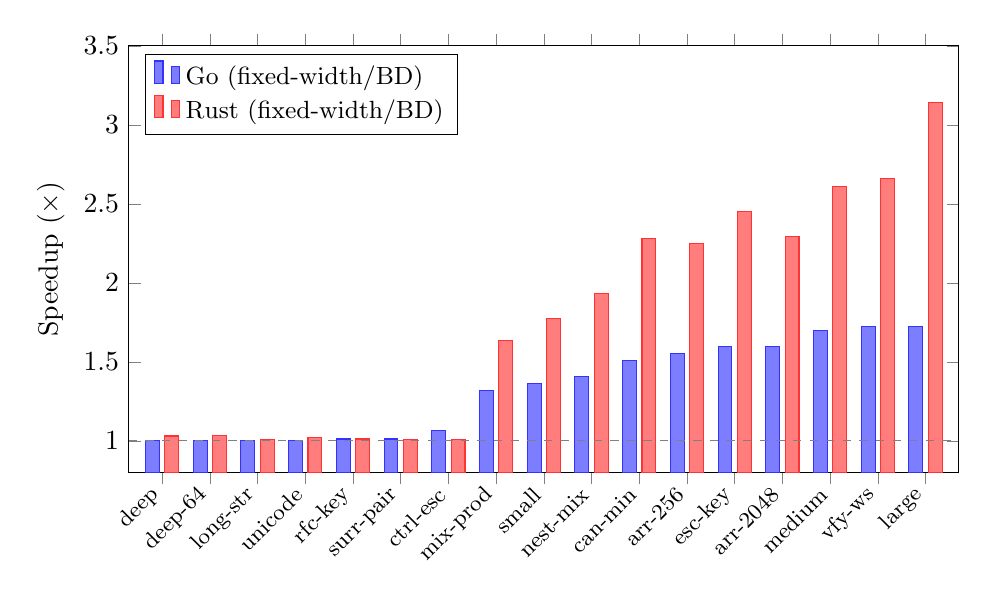
\begin{tikzpicture}
\begin{axis}[
    ybar,
    bar width=5pt,
    width=\textwidth,
    height=7cm,
    ylabel={Speedup ($\times$)},
    xtick={1,2,3,4,5,6,7,8,9,10,11,12,13,14,15,16,17},
    xticklabels={
        deep,
        deep-64,
        long-str,
        unicode,
        rfc-key,
        surr-pair,
        ctrl-esc,
        mix-prod,
        small,
        nest-mix,
        can-min,
        arr-256,
        esc-key,
        arr-2048,
        medium,
        vfy-ws,
        large},
    x tick label style={rotate=45, anchor=east, font=\footnotesize},
    ymin=0.8,
    ymax=3.5,
    xmin=0.3, xmax=17.7,
    ytick={1.0, 1.5, 2.0, 2.5, 3.0, 3.5},
    legend style={at={(0.02,0.98)}, anchor=north west, font=\small},
    legend cell align={left},
    every axis plot/.append style={fill opacity=0.85},
    clip=false,
]
% Go within-language (schubfach-vs-bd), sorted by Go speedup
% Pure-numeric outliers (numeric-boundary, number-heavy) shown separately in §8.5
\addplot[fill=blue!60, draw=blue!80] coordinates {
    (1, 1.000)
    (2, 1.000)
    (3, 1.001)
    (4, 1.003)
    (5, 1.012)
    (6, 1.012)
    (7, 1.065)
    (8, 1.320)
    (9, 1.364)
    (10, 1.408)
    (11, 1.509)
    (12, 1.552)
    (13, 1.595)
    (14, 1.599)
    (15, 1.698)
    (16, 1.721)
    (17, 1.724)
};
% Rust within-language (schubfach-vs-bd)
\addplot[fill=red!60, draw=red!80] coordinates {
    (1, 1.031)
    (2, 1.034)
    (3, 1.008)
    (4, 1.022)
    (5, 1.012)
    (6, 1.011)
    (7, 1.006)
    (8, 1.633)
    (9, 1.776)
    (10, 1.933)
    (11, 2.281)
    (12, 2.247)
    (13, 2.450)
    (14, 2.292)
    (15, 2.611)
    (16, 2.662)
    (17, 3.142)
};
\legend{Go (fixed-width/BD), Rust (fixed-width/BD)}
% Reference line at 1.0x
\draw[dashed, gray, thin] (axis cs:0.3,1.0) -- (axis cs:17.7,1.0);
\end{axis}
\end{tikzpicture}
\caption{API benchmark speedup of fixed-width over \burgerdybvig by
workload (canonicalize mode, \schubfach shown as representative;
\ryualg and \dragonbox produce equivalent ratios per
\S\ref{sec:results}).  Workloads sorted by Go speedup.  Values
above the dashed line indicate the fixed-width algorithm is faster.
Two pure-numeric workloads (\texttt{numeric-boundary} and
\texttt{number-heavy}) are presented separately in
\S\ref{sec:discussion} due to their degenerate number density
($\nu = 100\%$).  Number-dense workloads (right side) show the
largest advantage in both languages, consistent with a shared
algorithmic cause rather than language-specific runtime effects.}
\label{fig:api-speedup}
\end{figure*}
